%% sample template file for a MSc Thesis
%% The default is with two sided setup:
\documentclass[%
oneside,    %% uncomment for onesided layout
project,    %% uncomment not thesis but project report
nosummary   %% uncomment if no summary page should be generated
]{USN-MSc}

% The following command removes the chapter names form the header
% (comment/remove) if you prefer to have them:
\pagestyle{plain}

% --- Bibliography setup ---
%%% default is the "ieee" style
\usepackage[style=ieee, sorting=none]{biblatex}
%%% If you want to use "author-year" style
%%% where `\cite{Foo2011}` generates "Foo et al. (2011)"
%%% and   `\parencite{Foo2011}` generates "(Foo et al. 2011)"
%%% then comment the line above and use
%\usepackage[style=authoryear]{biblatex}
%%% or
%%% if you want to use "alphabetic" style then use
%%% where `cite[Foo2011]` generates "[Foo11]"
%%% then comment the line above and use
%\usepackage[style=alphabetic]{biblatex}
%%% instead.
%% load the bib file:
\addbibresource{MScThesis.bib}

\usepackage{lipsum} % just for providing fill text used in this template
\usepackage{array} % for adjusting tables?
\usepackage{pdflscape} % for landscape pages

%These two are used to add frames to figures.
\usepackage{graphicx}
\usepackage[export]{adjustbox}

% --- general setup ---
%% Please fill in the following parameters:
\newcommand{\mytitle}{%
%% title:
Assignments for section 3 (W3.1-W3.5)
}

\newcommand{\mysubtitle}{%
%% master programme (for thesis only)
%% uncomment the appropriate one:
%%Electrical Power Engineering
%Energy and Environmental Technology
%Industrial IT and Automation
%Process Technology
}

\newcommand{\mykeywords}{%
%% keywords (for thesis only):
<keyword one, keyword two, \ldots>
}

\newcommand{\myauthor}{%
%% author(thesis) or group code (project):
223786 Lars Rikard Rådstoga
}

\newcommand{\myparticipants}{
%% group participants (for project only)
<First participant>\\
<Second participant>\\
<Third participant>\\
<Fourth participant>
}

\newcommand{\supervisor}{%
%% supervisor:
<Supervisor's Name>}

\begin{document}

% --- title page setup ---
%\USNtitlepage%
%%% Please provide the following information:
%%% #1 optional figure (set to {} if not wanted)
%{%
%  {\normalsize}
%  \begin{figure}[!ht]
%    \centering
%   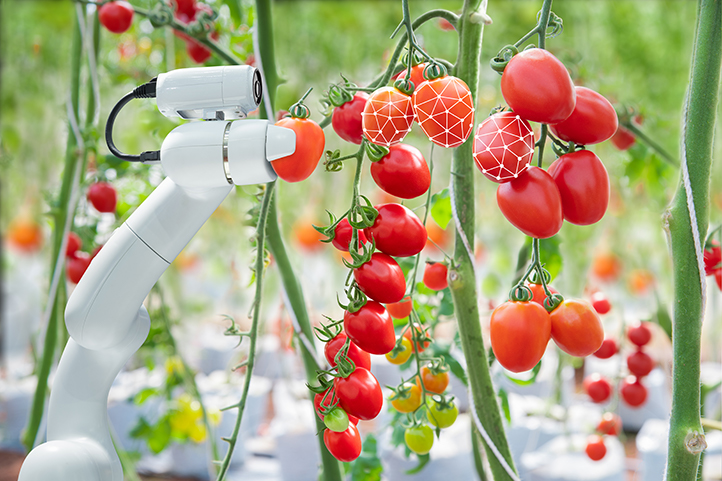
\includegraphics[width=0.8\textwidth]{TomatoPickerBot}
%   \label{fig:tomatoBot}
% \end{figure}
%}
% --- title page setup ---
\USNtitlepage%
%% Please provide the following information:
%% #1 optional figure (set to {} if not wanted)
{%
  {\normalsize}
   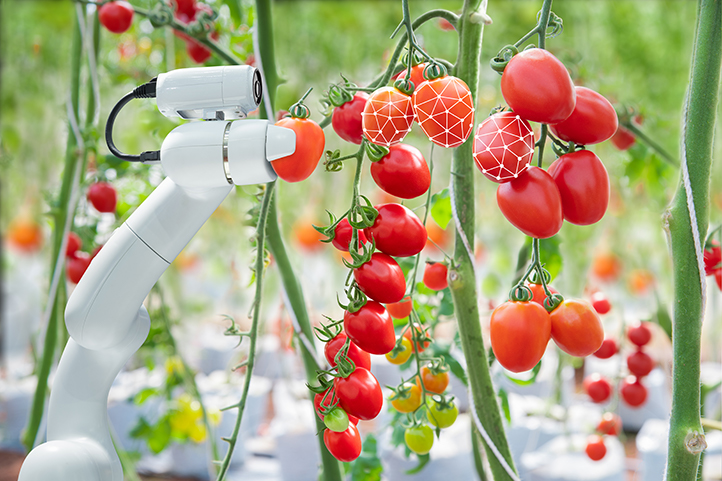
\includegraphics[width=\textwidth]{TomatoPickerBot}}
%% #2 Project partner:
{<Project partner>}
%% #3 Summary:
{%
\lipsum[6-7]
}


%\chapter*{Preface}
%\label{ch:preface}
%\addcontentsline{toc}{chapter}{Preface}
%\lipsum[1-3]
%\bigskip
%Porsgrunn, \today

%\myauthor %% for thesis
%\myparticipants %% for project


%% table of contents
\tableofcontents
\addcontentsline{toc}{chapter}{\contentsname}

%\listoffigures % out-comment if unwanted
%\addcontentsline{toc}{section}{\listfigurename}

%\listoftables  % out-comment if unwanted
%\addcontentsline{toc}{section}{\listtablename}

\chapter{System diagram for the chosen autonomous system}
\label{ch:sysDiagram}
This chapter contains context of the autonomous fruit picker system. Briefly discussing why it should be an autonomous system and how it should be organized in terms of building blocks and how data should flow through the system.
\section{Introduction of the system}
The autonomous fruit picker system is meant to be a contribution to combat increasing shortage in labor in the agricultural landscape. As fruit picking is tedious and back-breaking work it is not the most lucrative profession. Most robotized fruit-picking solutions as of today involve augmentation of the farming environment to a great degree, such as moving the operation in-doors or levitating the farming beds. Perhaps these augmentations are advantageous for tackling multiple challenges, but they might have their downsides as well. Today we are going to assume that traditional outdoor ground farming is the most popular practice and will remain that way for most of the foreseeable future. The target environment for the system will therefore be a more rugged and unpredictable one compared to environments in which existing solutions operate.
\section{System diagram}
Based on system architecture theory from the book Introduction to AI Robotics \cite{murphy2000introduction}, the system will be organized by the five subsystems as seen in figure \ref{fig:sysDiagram}.
\begin{figure}[!ht]
  \centering
  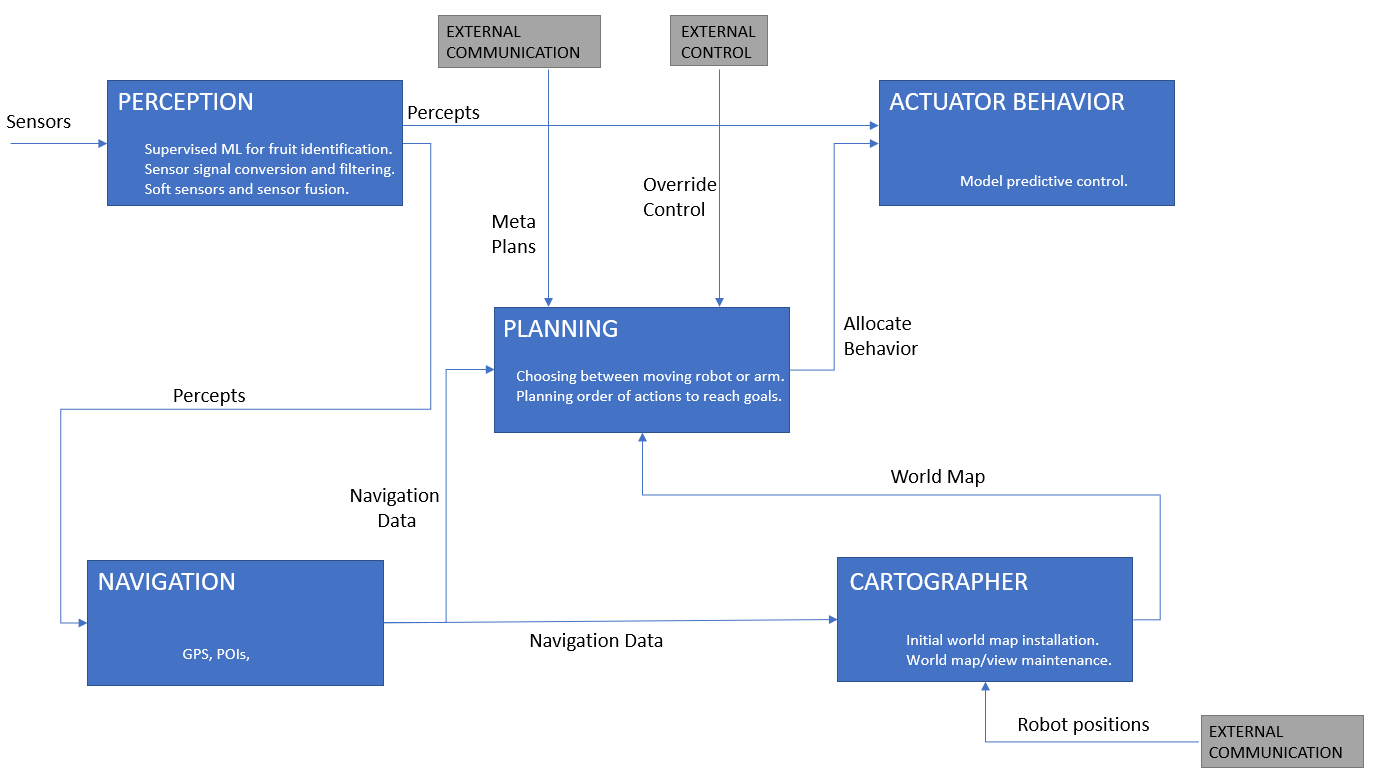
\includegraphics[width=0.95\textwidth, frame]{SystemDiagram}
  \caption{System diagram with focus on data input and internal data flow. \cite{murphy2000introduction}}
  \label{fig:sysDiagram}
\end{figure}
In order for a system to traverse a world, several cognitive modules need to cooperate. As described in the literature, there are usually a minimum of five of these modules or subsystems: perception, navigation, planning, cartographer, and motor schema. In the aforementioned system diagram, shown in this paper, motor schema is instead named actuator behavior. These subsystems will be made up of one or more classes in object-oriented programming. For this solution it is plausible that different implementations of these subsystems will be required for the robot's main body and the gripper-equipped arm.

The perception subsystem is tightly-knit together with the sensor inputs. Sensors will supply the system with a continuous stream of information about the surrounding world: tactile feedback, LIDAR, camera, GPS, wheel rotation encoder, and more. Analog data will have to be converted to digital and raw data will need to be filtered. Redundant sensors can be combined to increase accuracy or different kinds of sensors can be combined: fused. ML models trained for identification can also be part of this subsystem. Most important is the model for identifying and differentiating fruit.

The navigation subsystem will be responsible for planning and monitoring movement of the robot. This module will however require data from related modules: transformed sensor data from the perception module, map data from the cartographer and plans from the planning module. Initially the planning module will decide where the robot should move, the cartographer will have partial data about surrounding world. The navigation module will use this data to calculate and iteratively re-calculate optimal paths. If the cartographer discovers some obstacles in the way of the planned path the navigator might require major re-routing. Additionally, perceptive signals can be used directly for collision detection. If something unexpected moves in the way of the robot, the sensors will pick this disturbance up before it is mapped by the cartographer.

The planning subsystem will be the main local decision maker for the robot. Its main tasks involve planning such as what area to pick fruit from during spans of hours, managing the order of main activities such as moving to a bush, drop-off area, picking fruit, charging, and more. A more macro level of decision-making is made in a centralized server, so this will be important inputs for the module. But it will also need to look at perception data, such as how many fruit are visible, to e.g. micromanage between moving the robot and picking fruit. Such information will also be communicated to the server to further adjust macro management.

The cartographer subsystem will both use perceptive data to map the world, but it will also communicate with other units through the central server to build a more detailed map.

The actuator subsystem will use both navigation data, perceptive data and control algorithms such as PID, LQI, or MPC to control the robot.

\chapter{How to organize software for autonomous systems}
\label{ch:softOrganz}
This chapter contains information on the organization of software in the autonomous system.
\section{Reflection}
The system will be distributed into three different layers, see figure \ref{fig:layers}.
From the ground-up: multiple robots can operate independently and run their own code, a common server will be the responsible for macro planning, communication between robots, collecting data, training ML models and distributing updated software. Additionally, the system requires a database for saving sensory data, world views, and other resources that can be used to further improve the system or that create value in other ways.

\begin{figure}[!ht]
  \centering
  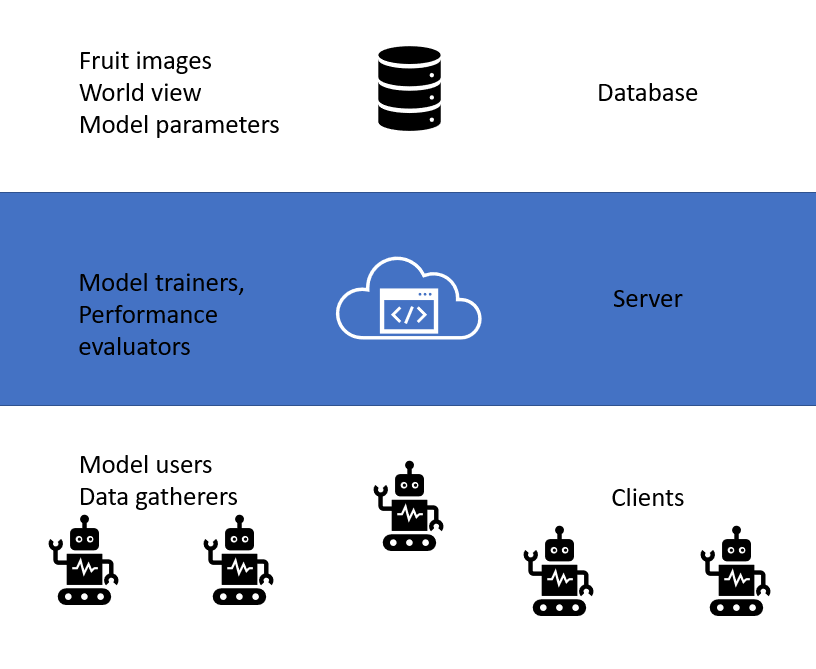
\includegraphics[width=0.80\textwidth, frame]{SystemLayers}
  \caption{Layered architecture displaying multiple robots communicating through a common server and database.}
  \label{fig:layers}
\end{figure}

\chapter{Information collection}
\label{ch:infoCol}
This chapter contains a discussion on collection of information.
\section{Reflection}
Information collection is a crucial aspect of autonomous systems, particularly for tasks that require precise sensing, planning, and acting. In the context of the autonomous fruit-picking system, effective information collection would involve the use of sensors to accurately detect and identify fruit on a plant, as well as to gather information about the surrounding environment. This information would be used to generate a plan for the robot to safely and efficiently pick the fruit, while also avoiding obstacles and potential hazards.

One of the key challenges in information collection for an autonomous fruit picking system is ensuring the accuracy and reliability of the data being gathered. This may involve the use of multiple sensors, as well as algorithms and machine learning techniques to process and interpret the data. It is also important to consider the privacy and security of the data being collected, particularly if the system is being used in a public or sensitive location.

To address these concerns, it may be necessary to implement measures such as encryption and secure storage for the data collected by the system. It may also be necessary to consider the potential risks and impacts of data collection on individuals and communities, and to put in place appropriate safeguards and policies to protect privacy and ensure the responsible use of the data.

AI algorithms can be a potential solution to the problem. Enabling automatic detection and obscure identifiable features such as faces, license plates, and other identifying characteristics. This can be done using techniques such as deep learning and pattern recognition, which can help to identify and anonymize these features even when they are partially obscured or occluded. As seen previously in Figure \ref{fig:layers}, it is thought to save sensory data in a centralized database, tasks like anonymizing data can be done on the server level, before it is saved to the database.

The collected data can be used to improve the machine learning (ML) models used by the system in a number of ways. First, the data can be used to train the ML models, allowing them to become more accurate and reliable over time. Second, the data can be used to identify patterns and trends in the environment that may not be immediately obvious, which can be used to optimize the robot's operation and improve its efficiency. Finally, the data can be used to fine-tune the ML models, making them more robust and able to handle a wider range of situations.

\chapter{Learning}
\label{ch:learn}
This chapter contains a reflection on the use of learning in the autonomous system.
\section{Reflection}
Machine learning is a subset of artificial intelligence that involves the use of algorithms and statistical models to enable computers to learn and make predictions or decisions without explicitly being programmed to do so. It can be used to identify fruits and other parts of plants, it can be used to control the robots' various actuators, and more.

\section{Identification}
One way machine learning can be used for fruit identification is through the use of image recognition algorithms. These algorithms can be trained on a large dataset of images of different types of fruit, along with corresponding labels identifying the type of fruit in each image. The algorithm can then be fed new images and will use the patterns it learned from the training data to classify the fruit in the new images. This can be done in real-time, for example, by using a camera to take a picture of a fruit and using the machine learning model to identify it.

In addition to fruit, the robot should be trained to recognize and array of things to be able to operate: Plants, paths and crop rows, weeds, landmarks, and more.

\section{Datasets}
A good dataset for training image identification models needs to be diverse, representative, and balanced to produce good results.

Diversity refers to the range of different types of images that are included in the dataset. A diverse dataset will include a wide variety of images that are representative of the types of images the model will be expected to classify in the real world. E.g., a dataset for training a model to identify different types of fruit should include images of fruit from different angles, in different lighting conditions, and in different stages of ripeness.

Representativeness refers to the extent to which the images in the dataset accurately reflect the real-world distribution of the types of images the model will be expected to classify. Since the model will be used to identify fruit in a field, fruit hanging on stems, the dataset should include a representative sample of fruit that are found in an orchard.

Balance refers to the distribution of different types of images within the dataset. A balanced dataset will have roughly equal numbers of images for each class the model is expected to classify. This is important because if the dataset is heavily skewed towards one class, the model may be biased towards that class and may perform poorly on images from other classes. In this case the model should be trained for identification of all useful classes of the fruit plant: fruit, stems, leaves, flowers, and more.

In addition to these factors, it is also important that the images in the dataset are of high quality and correctly labeled. Poor quality images or incorrect labels can lead to a model that is poorly trained and performs poorly on real-world data. Premade datasets likely exist, but should be fitted and supplemented with new data gathered by the robots and labeled by human operators.

Overall, a good dataset for training image identification models should be diverse, representative, and balanced, and should consist of high quality images that are correctly labeled.

\section{Reinforcement}
Reinforcement learning is a type of machine learning that involves training a model to learn a policy for taking actions in an environment in order to maximize a reward. Both reinforcement learning and image recognition can be used in combination with sensory inputs such as LIDAR and odometers to control the movements of a robot in order to reach its goals.

By combining reinforcement learning, image recognition, and sensory inputs such as LIDAR and odometers, a robot can use its vision and its understanding of the environment to make more informed decisions about its movements and to learn a policy for achieving its goals. For example, a robot equipped with image recognition and LIDAR could use its vision to identify the location of a specific object within an image, and then use its LIDAR data to determine the best path to reach that object. The robot could then use reinforcement learning to learn a policy for selecting actions that are likely to lead it to the object, based on the rewards it receives for successfully reaching the object or for making progress towards the object.

% A dummy command that causes all bibliographyentries to be displayed
% even though there were not cited in the document. Used for demonstration
% purposes only in this template file.
~\nocite{*}

\cleardoublepage

% The bibliography should be displayed here...
%\printbibliography[heading=bibintoc]
% You rather like to call the bibliography "References"? Then use this instead:
\printbibliography[heading=bibintoc, title={References}]


%\appendix
%\renewcommand{\appendixname}{Paper} %% So we get 'Paper X' displayed instead


%\chapter[Short Title of Paper A]{Title of Paper A (probably very long and therefore not good to have in the header)}
%\label{paper-a}
%
%\paragraph{Note}
%Since some papers tend to have a rather long title it is good to provide the optional short title which then will be displayed in the table of contents and header instead of the long original title.
%On the openening page of the chapter the orginal \emph{long} title will be displayed.\bigskip
%
%\emph{Short descriptive text of paper follows here.}\bigskip
%
%The paper itself needs to be included in the published form as PDF on the next pages.
%This can be done using the \texttt{pdfpages} package by adding the command:
%
%\begin{verbatim}
%\includepdf{pages=-,openright}{Filename}
%\end{verbatim}
%
%You can omit the \texttt{.pdf} when specifying the \texttt{Filename}. Also you should include always include the option \texttt{openright} since it would look strange to have the paper starting at the back of the cover page.
%
%There are more options like only adding specific pages:
%\begin{verbatim}
%\includepdf{pages=2-6,openright}{Filename.pdf}
%\end{verbatim}

%For more options see Appendix~\ref{paper-b} where the most important pages of the \texttt{pdfpages} manual were inlcuded using \texttt{pdfpages}.


%%% Command to include a PDF file directly including all pages:


%\chapter[Short Title of Paper B]{Title of Paper B}
%\label{paper-b}
%Short descriptive text of paper follows here.
%
%Here we included the first five pages of the \texttt{pdfpages} manual itself.
%
%\includepdf[pages=1-5,openright]{fig/pdfpages}
%
\end{document}

%%% Local Variables:
%%% mode: latex
%%% TeX-master: t
%%% End:
